\begin{figure}[!t]
	\centering
	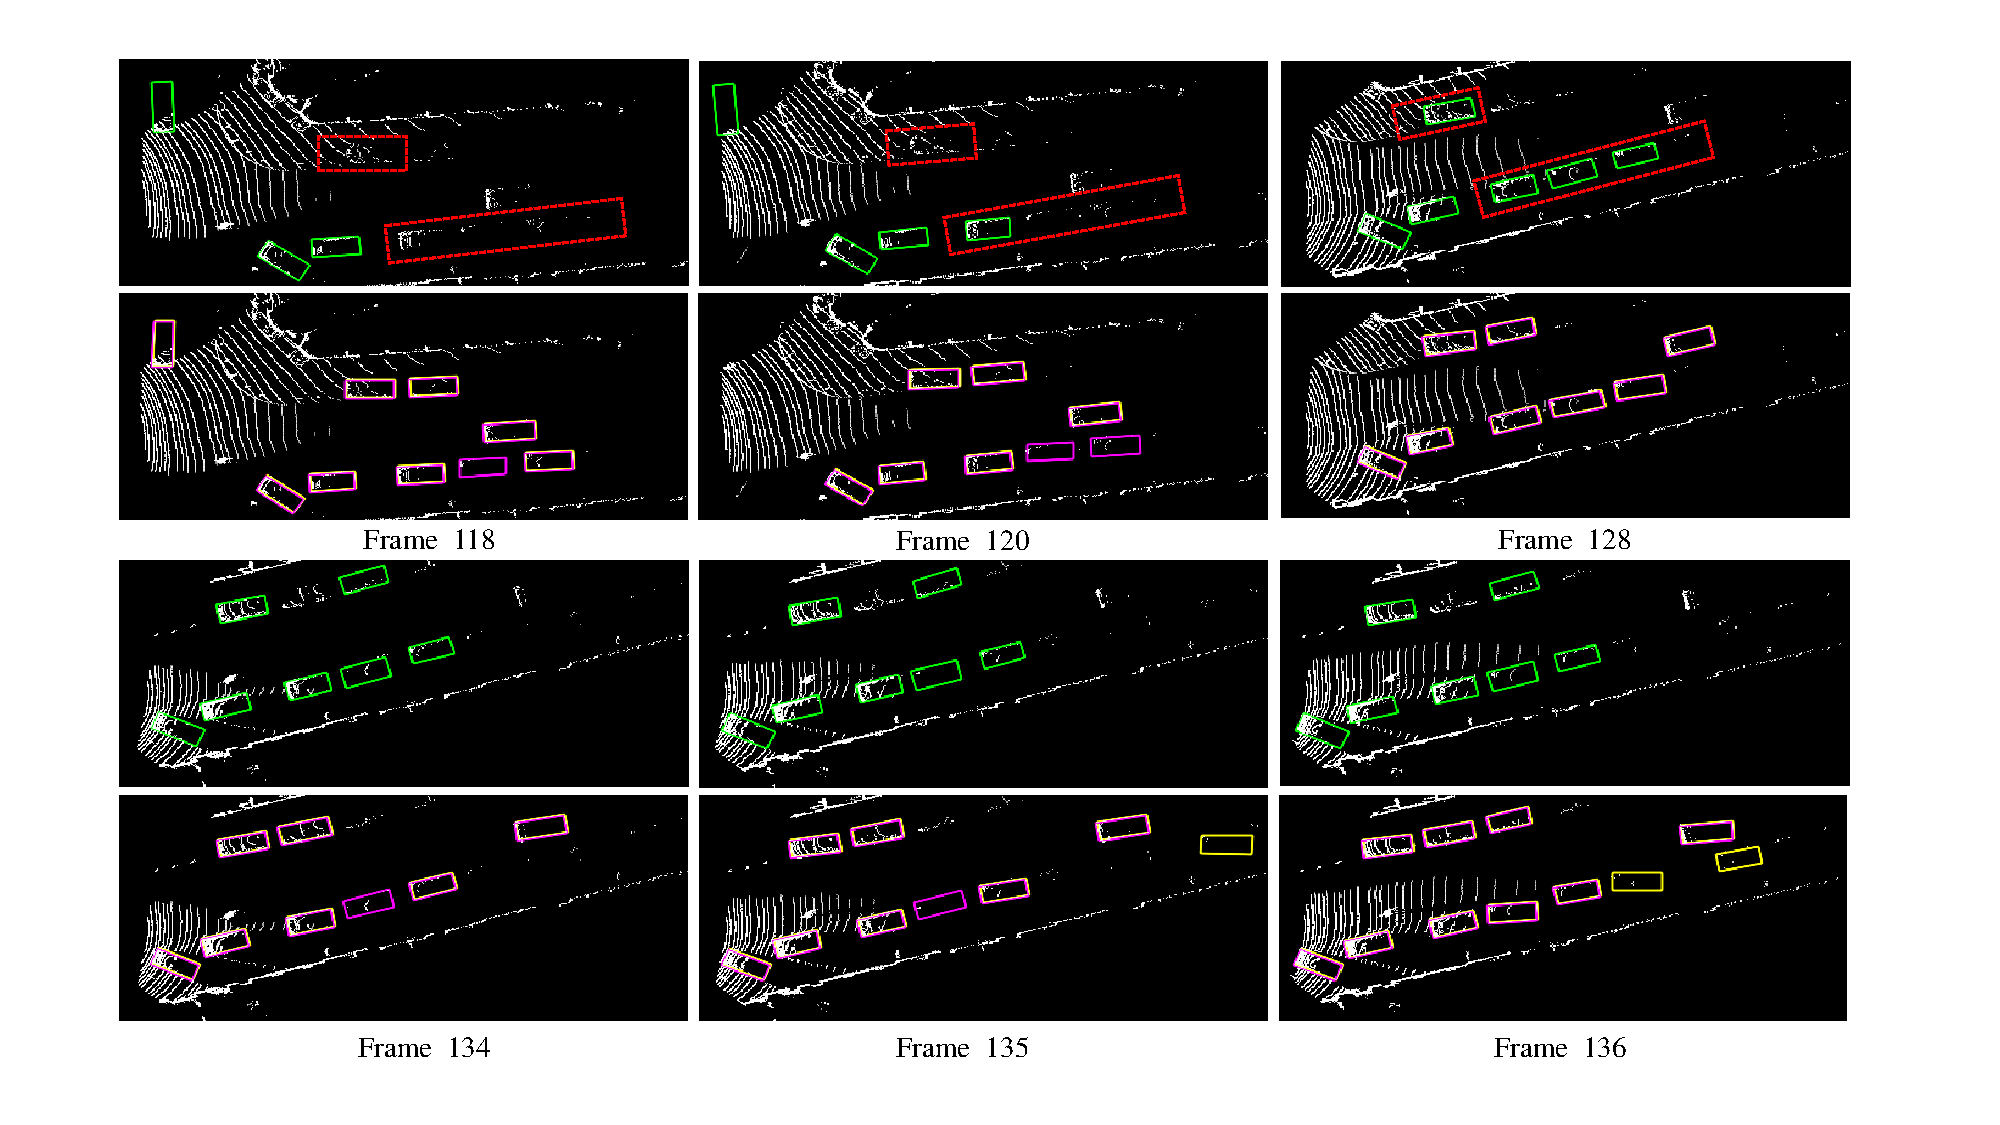
\includegraphics[trim={2cm, 1cm, 2.5cm, 1cm}, clip, width=\textwidth]{./imgs/examples.pdf}
	\vspace{-1.0cm}
	\caption{视频序列0的标签以及预测结果可视化。\textcolor{green}{绿色}为官方提供的标签框, \textcolor{yellow}{黄色}是时序步长$\tau = 1$的预测结果,\textcolor{magenta}{洋红色}为时序步长$\tau = 3$的预测结果。混合颜色的框是黄色框和洋红色框重叠造成的,最好彩色打印查看。}
	\label{fig:examples}
\end{figure}
